\documentclass[12pt]{article}
\usepackage{amsfonts,amssymb,amsmath}
\usepackage{graphicx}
\usepackage{listings}

\begin{document}
{\Large\bf PROJECT 1: READ ME FILE \\
\vspace{0.5cm}}\\[10pt]
Francine Leech, Reffat Manzur, Chen Xiang 

\subsection*{P1}
(1) 
The \textit{CubicBezier.m} plots a cubic spline specified by a sequence of de Boor controls points from the user. The user presses enter to indicate all the desired points have been selected. 
\\
For example if we input 7 points, the graph we get is:\\ 
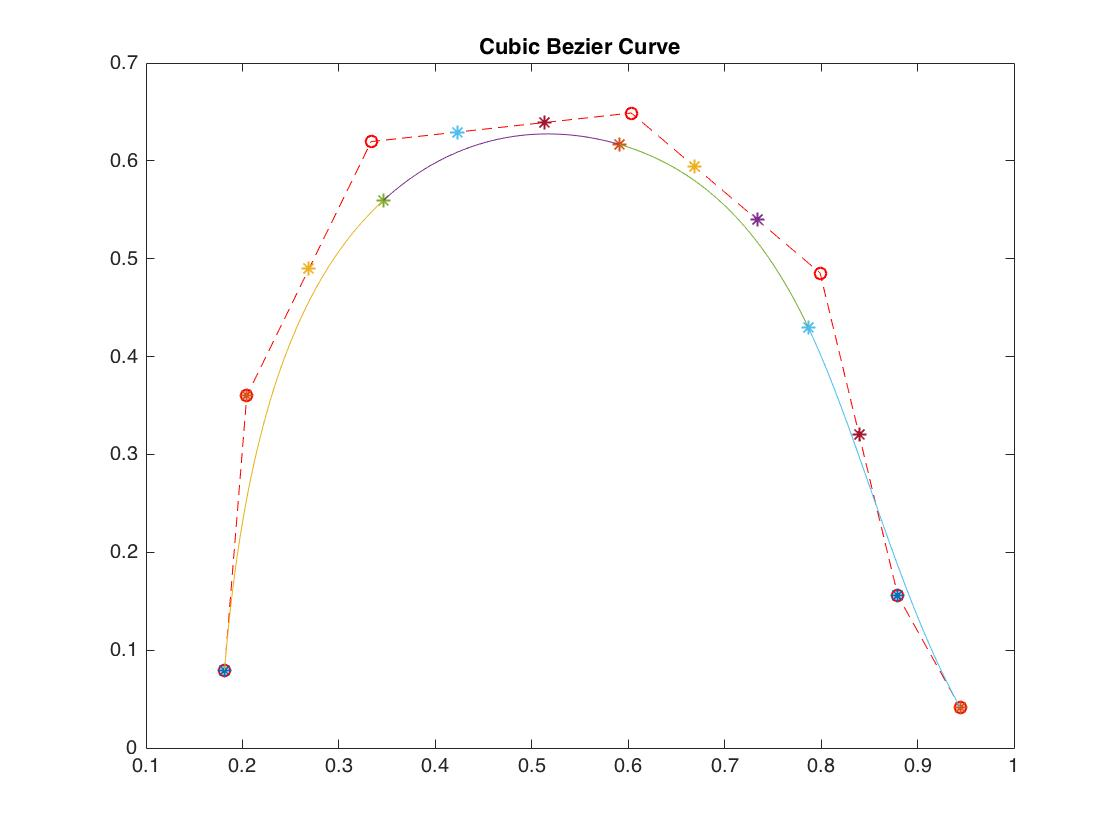
\includegraphics[scale=.25]{CubicGraph}

\subsection*{P2}
(2) 
The \textit{drawDE.m} uses the de Casteljau subdivision method and  yields a polygonal line which approximates \textit{Bezier curve}. The variable $n$ is the number of iterations and $t$ is the size of the subdivision. The user presses enter to indicate all the desired points have been selected. 
\\
For example if we input $n = 5 , \; t = \frac{1}{2}$ and a series points through screen: 

\begin{lstlisting}[language=Matlab]
n = 5; 
t = 1/2; 
%% User input of the data
[x,y] = ginput();  
d = [x,y]; % d(i,:) i = 1,2,.. represents a point 
d = sortrows(d); % sort our data 
%% Run the subdivision and draw curve
b = calculateDE(d, n, t); 
% calculate the points used to draw the curve 
b = sortrows(b); % sort our data 
plot(d(:,1), d(:,2), 'r*'); % draw the input data d
hold on;
plot(b(:,1), b(:,2), 'b-') % draw our curve 
title('Bezier Curve')
\end{lstlisting}
Then we can get the graph: \\
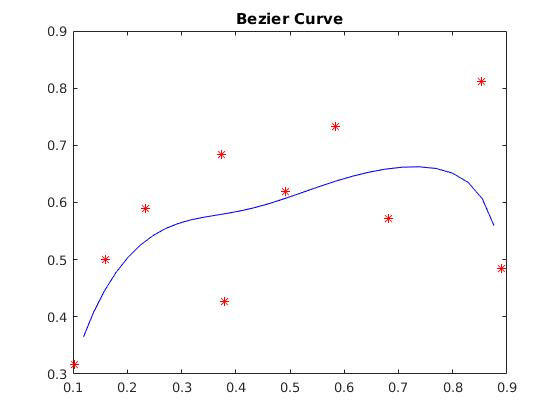
\includegraphics[scale=.5]{npoints}
\end{document}